\documentclass[border=1mm]{standalone}
\usepackage{tikz}
\begin{document}
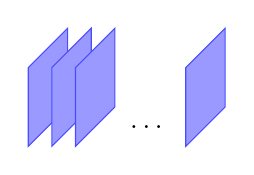
\begin{tikzpicture}
\coordinate (origin) at (0, 0);
\coordinate (upper) at (0, 1);
\coordinate (bleft) at (.5, .5);
\coordinate (uleft) at (.5, 1.5);
\draw [-, blue!70!white, fill=blue!40!white] (origin) -- (upper) -- (uleft) -- (bleft) -- cycle;

\pause

\coordinate (origin) at (.3, 0);
\coordinate (upper) at (.3, 1);
\coordinate (bleft) at (.8, .5);
\coordinate (uleft) at (.8, 1.5);
\draw [-, blue!70!white, fill=blue!40!white] (origin) -- (upper) -- (uleft) -- (bleft) -- cycle;

\pause

\coordinate (origin) at (.6, 0);
\coordinate (upper) at (.6, 1);
\coordinate (bleft) at (1.1, .5);
\coordinate (uleft) at (1.1, 1.5);
\draw [-, blue!70!white, fill=blue!40!white] (origin) -- (upper) -- (uleft) -- (bleft) -- cycle;

\node (dots) at (1.5, .25) {$\dots$};

\coordinate (origin) at (2, 0);
\coordinate (upper) at (2, 1);
\coordinate (bleft) at (2.5, .5);
\coordinate (uleft) at (2.5, 1.5);
\draw [-, blue!70!white, fill=blue!40!white] (origin) -- (upper) -- (uleft) -- (bleft) -- cycle;

\end{tikzpicture}
\end{document}